\chapter{Analýza a návrh řešení}
Analýza a návrh implementace (včetně diskuse různých alternativ a volby implementačního prostředí).

Tato kapitola se dělí na analýzu a návrh. V analýze se zaměřilo na prostudování tří existujících řešení. Z informací získaných z dokumentace jsem sestavil návrh pro Ruby ACL.


\section{Analýza}

Protože práce byla velmi přesně zadána, nezbylo příliš prostoru na různé alternativy. Ruby bylo zadáno jako implementační prostředí. Způsob zpracování byl zadán pomocí ACL - Access Control List. Hlavním úkol bylo zjistit, jakým způsobem implementovat samotné ACL a řádně implementaci zdokumentovat a otestovat.

\subsection{Exitující řešení}
\label{sec:anal-existujicireseni}

Při řešení vlastního návrhu na model řízení přístupových práv jsem vycházel ze dvou zdrojů – známých řešení a jednoho obecného řešení.

\subsubsection{Obecné řešení}
Obecným řešením je držet si tabulku, kde ve sloupcích budou objekty, ke kterým je možno přistupovat a v řádcích jsou přistupující. V poli pak jsou hodnoty boolean, které vyjadřují buď allow nebo deny. Příklad tabulkového řešení je v tabulce \ref{tab:tab2}.
TODO prelozit do cestiny
\begin{table}%[h]
\centering
%% Some packages, such as MDW tools, offer better commands for making tables
%% than the plain LaTeX2e tabular which is used here.
\begin{tabular}{|r||c|c|c|}
\hline
Who / Where & Surgeryroom & ambulance & Patient's room\\
\hline\hline
Doctors & 1 & 1 & 1\\
\hline
Nurses & X & 1 & 1\\
\hline
Patients & X & X & 1\\
\hline
\end{tabular}
\caption{Obecné řešení modelu práv pomocí matice}
\label{tab:tab2}
\end{table}

%-------------------------------------

\subsubsection{Oracle}
Jedním z řešení je podnikové řešení prezentované v Oracle® XML DB Developer's Guide, 11g Release 1 (11.1), Part Number B28369-04 na stránkách Oracle dokumentace \cite{oracle}. Ve stati Access Control Lists and Security Classes je popsán koncept firmy ORACLE.
 
Text popisuje několik podmínek a pojetí řízení přístupu. Každá z popsaných entit, uživatel, role, privilegia, bezpečnostní třídy, Access Control List (ACL) a Access Control Entry (ACE), je realizována deklarativně jako XML dokument nebo fragment.  

Bezpečnostní autorizace vyžaduje definovat, kteří uživatelé, aplikace nebo funkce mohou mít přístup k jakým datům nebo jaké druhy operací mohou provádět. Existují tedy tři dimenze: (1) kteří uživatelé mohou, (2) vykonávat jaké činnosti, (3) na jakých datech. V souvislosti s každou jednotlivou dimenzí hovoříme o (1) principals - zmocnitelích, (2) privileges - oprávněných, a (3) objektech, které korespondují s těmito třemi dimenzemi. Principals mohou být uživatelé nebo role/skupiny.

Principals a privileges (dimenze 1 a 2) jsou deklarativním způsobem spojeni v definovaných seznamech řízení přístupu - ACL. Ty jsou pak spojené s třetí dimenzí - daty, různými způsoby. Například úložiště zdrojů nebo tabulky dat Oracle XML DB mohou být ochráněny pomocí PL / SQL procedury DBMS\_XDB.setACL nastavením jeho řídícího ACL.

%-------------------------------------

\subsubsection{phpGACL}
Druhým ze zdrojů, z nichž jsem vycházel, je řešení prezentované v Generic Access Control List with PHP - phpGACL na \cite{phpGACL}.

Nástroj phpGACL je sada funkcí, která umožňuje použít řízení přístupu na libovolné objekty (webové stránky, databáze, atd.), jiným libovolným objektům (uživatelé, vzdálené počítače, atd.). 
Stejně jako Oracle nabízí jemně nastavitelnou kontrolu přístupu s jednoduchou a velmi rychlou správou. Je napsán v populárním dynamickém skriptovacím jazyku PHP.

Nástroj phpGACL vyžaduje relační databáze pro ukládání informací k řízení přístupu. Přistupuje k databázi prostřednictvím tzv. abstraktního obalu ADOdb. Je kompatibilní s databázemi, jako PostgreSQL, MySQL a Oracle. 

Nástroj phpGACL používá pojmy jako ACO a ARO:
\begin{itemize}
\item Access Control Objects (ACO), jsou věci, ke kterým chceme ovládat přístup (např. webové stránky, databáze, pokoje, atd.).
\item Access Request Objects (ARO), jsou věci, které žádají o přístup (např. osoby, vzdálené počítače, atd.)
\item ARO stromy definují hierarchii skupin a ARO. Skupiny mohou obsahovat jiné skupiny a ARO.
\item Výchozí "catch-all" politikou stromu ARO je vždy "DENY ALL ".
\item Chceme-li přiřadit přístupovou politiku ve stromu směrem dolů, explicitně přiřazujeme oprávnění skupinám a ARO pro každou ACO, pro kterou je potřeba.
\end{itemize}

\section{Návrh implementace}
Nechal jsem se inspirovat jak Oraclem tak phpGACL. Oba modely řízení přístupových práv mají podobnou strukturu nebo stejnou s jiným pojmenováním. Z Oraclu jsem převzal koncept a pojmenování dimenzí: principals, privileges, objects, ze kterých jsem vytvořil hlavní třídy. 

Jemně nastavitelných přístupových práv se docílí pomocí Access Control Listu. ACL obsahuje seznam pravidel jednotlivých přístupů. Pravidlo se nazývá Access Control Entry (ACE). V ACE je uloženo \underline{kdo}, nebo \underline{co} má jaká \underline{práva} přistupovat k jakým \underline{objektům}. Těmto třem rozměrům se v problematice přístupových práv říka: principals, privileges, resource objects.



\subsection{Rozhraní}

S knihovnou RubyACL je zapotřebí nějak komunikovat. Za účelem vytvoření a nastavení zmoctnitelů, oprávněních, zdrojových objektů a pravidel musí uživatel předat knihovně potřebné vstupy popsané v tabulce. Hlavní účel knihovny je rozlišit jestli někdo nebo něco má oprávnění na nějaký cílový objekt. Pokud zmocnitel má nebo nemá přístup se uživatel dozví podle výstupu. Výstupem je true nebo false hodnota. \ref{tab:tab3} TODO přidat do tabulky i popis
Model rozhraní se nachází v příloze jako obrázek \ref{}


\subsubsection{Rozhraní mezi Ruby-ACL a databází}
RubyACL bylo testováno s databází eXist-db, se kterou komunikovalo pomocí eXistAPI. 
K používání RubyACL s jinou XML databází než eXist je zapotřebí komunikační rozhraní, které nahradí eXistAPI. 
V ukázkové třídě API je výčet všech potřebných metod, které RubyACL používá, včetně parametrů a výstupů. Je potřeba podle vzorové třídy API naimplementovat nové komunikační rozhraní. 



\subsubsection{Rozhraní mezi Ruby-ACL a uživatelskou aplikací}
Jedná se o výčet public metod třídy RubyACL.
...přidat výčet
Na této části záleží bezpočenost. Potencionálně nebezpečné místo k útoku.



\begin{table}[h]
\centering
\begin{tabular}{|c|c|}
\hline
\textbf{jméno} & \textbf{typ} \\
\hline
\multicolumn{2}{|l|}{Vstupy} \\
\hline
principal & string\\
\hline
privilege & string\\
\hline
resource object & string\\
\hline
\hline
\multicolumn{2}{|l|}{Výstupy} \\
\hline
access & boolean\\
\hline
\end{tabular}
\caption{Vstupy a výstupy knihovny}
\label{tab:tab3}
\end{table}

\subsection{Ukázka použití}
Tato sekce prezentuje stručné ukázky použití

\subsubsection{Příklad nastavení práv}

Příklad tohoto kódu v podstatě říká: Pokud metoda \verb|ac_check| vratí hodnotu true, přístup povolen a aplikace provede co zamýšlela provést. Pokud vrátí hodnotu false, tak je přístup zamítnut. Tento postup názorně vysvětluje obrázek \ref{fig:Communication diagram} zobrazující komunikaci a průběh jednoho dotázení na pravidlo.

\begin{lstlisting}
require 'eXistAPI'    #must require 'eXistAPI' to comunicated with eXist-db
#create instance of ExistAPI
@db = ExistAPI.new("http://localhost:8080/exist/xmlrpc", "admin", "password")    
@col_path = "/db/test_acl/"         #sets the collection where you want to have ACL in db
@src_files_path = "./src_files/"    #path to source files
@my_acl = RubyACL.new("my_acl", @db, @col_path, @src_files_path, true)
#it's good to create some principals at the begging
@my_acl.create_principal("Sheldon")
@my_acl.create_privilege("SIT")
@my_acl.create_resource_object("seat", "/livingroom/couch/Sheldon's_spot", "Sheldon")
@my_acl.create_ace("Sheldon", "allow", "SIT", "seat", "/livingroom/couch/Sheldon's_spot")
\end{lstlisting}


\subsubsection{Příklad kontroly práv}

Druhý příklad naznačuje použití metody pro vytvoření pravidla. Pro vytvoření pravidla musí existovat instance Ruby ACL. Metodě create\_ace aplikace předá uživatelské jméno zmocnitele, typ přístupu (allow nebo deny), oprávnění a požadovaný objekt.

\begin{lstlisting}[firstnumber=12]
#Next method in if returns deny
if(@my_acl.check("Penny", "SIT", "seat", "/livingroom/couch/Sheldon's_spot"))
	puts "Access allowed. You may retrive resource object."
else
	puts "Access denied."
\end{lstlisting}

\subsection{Use Case Scénáře}
%\begin{verbatim}\end{verbatim}
\subsubsection{Ověřování oprávnění k objektu}
Uživatel má vytvořenou instanci RubyACL, která pracuje s pravidly.
Hlavní úspěšný scénář:
\begin{enumerate}
\item Uživatel zavolá metodu acl\_check. Přes tuto metodu se dotáže knihovny, jestli uživatel/skupina (ne)mají oprávnění ke zdrojovému objektu.
\item a) Systém vrátí true v případě, že uživatel/skupina má specifikované nebo vyšší oprávnění.
\item b) Systém vrátí false v případě, že uživatel/skupina nemají specifikované nebo vyšší oprávnění.
\end{enumerate}
Rozšíření:

0a) Pokud neexistuje žádné pravidlo, systém vrátí false, protože nenašel, žádné vyhovující pravidlo.
%\begin{verbatim}\end{verbatim}

\subsubsection{Zadávání pravidla (ACE)}
Uživatel má vytvořenou instanci RubyACL, která obsahuje pravidla.
Hlavní úspěšný scénář:
\begin{enumerate}
\item Uživatel zavolá metodu set\_new\_ace a specifikuje údaje (Uživatel/skupina, typ přístupy (allow/deny), oprávnění, zdrojový objekt
\item Knihovna nastaví pravidlo a vrátí 0, když vše proběhlo v pořádku, a 1 když nastala chyba.
\end{enumerate}
Poznámka: Jde vlastně o přiřazování oprávnění uživatelům na objekt



%-------------------------------------



\subsection{Data flow diagram}
TODO smazat starý obrázek. Okomentovat nový
Data flow diagram (viz "Obrázek 2") znázorňuje tok dat mezi jednotlivými funkcemi aplikace. Popisuje funkce a jejich vazby. Uložiště pro ACL je používaná databáze. Pro každou databázi bude jedna instance Ruby-ACL.
\begin{figure}
%\centering
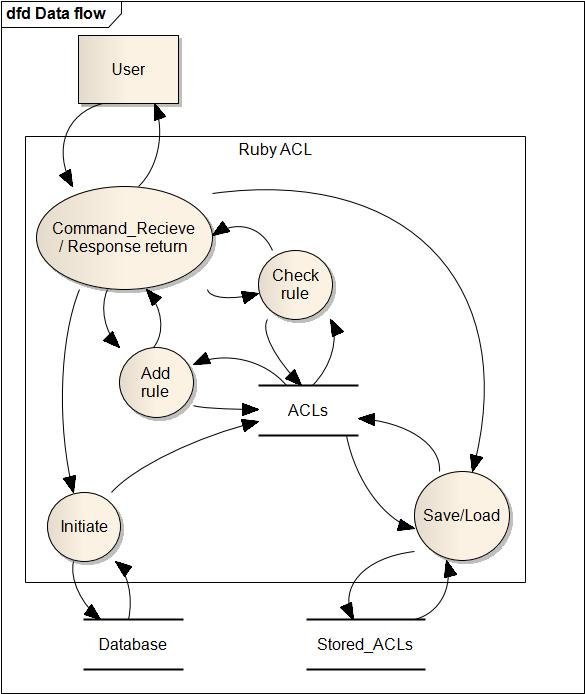
\includegraphics[width=15cm]{DataFlowBigFont.jpg}
\caption{Data flow diagram}
\label{fig:Data flow diagram}
\end{figure}
\begin{figure}
%\centering
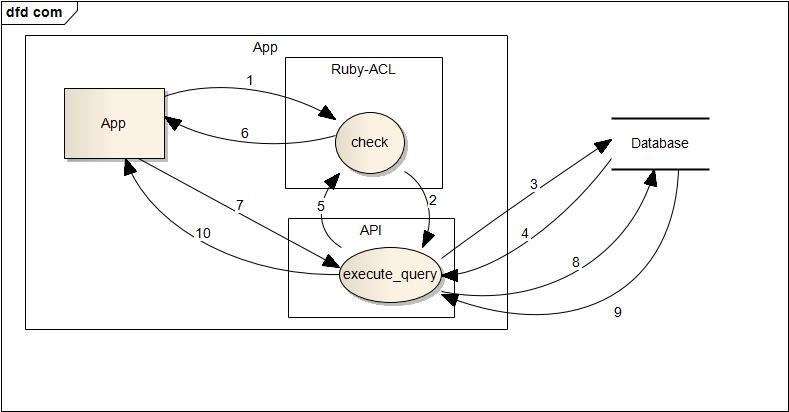
\includegraphics[width=15cm]{com.jpg}
\caption{Diagram znázorňující komunikaci}
\label{fig:Communication diagram}
\end{figure}

%-------------------------------------

\subsection{Class diagram}
Class diagram (viz "Obrázek 3") znázorňuje základní třídy aplikace a jejich vazby.
\begin{figure}
%\centering
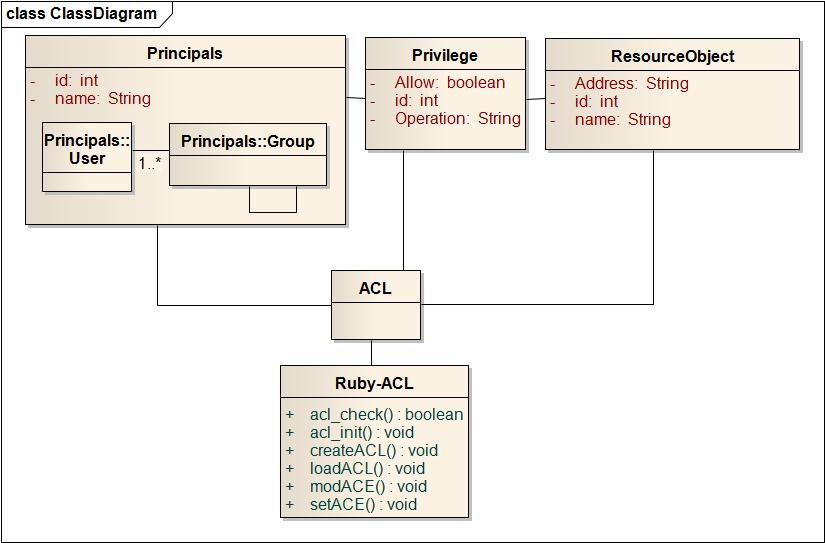
\includegraphics[width=15cm]{ClassDiagram2.jpg}
\caption{Class diagram}
\label{fig:Class diagram}
\end{figure}

%-------------------------------------
\section{Popis logiky vyhodnocování pravidel}
V této kapitole je popsáno jakým způsobem RubyACL rozhoduje o přidělení přístupu. Nejkonkrétněji se tímto zabývá sekce "Pravidla rozhodování", nicméně k pochopení celku je potřeba vědět vlastnosti jednotlivých objektů, které jsem nazval ACL objekty. O nich se dočtete ve stejnojmenné sekci.
Vše se odvijí od priority rozhodování.

\subsection{ACL Objekty}
ACL objekt je principal, který se dělí na individual a group, privilege

\subsubsection {Zmocnitel (Principal)}
Principal = [Individual, Group]
\begin{verbatim}
        <Group id="Administrators">
            <membership>
                <mgroup idref="ALL"/>
            </membership>
        </Group>
        <Individual id="sirljan">
            <membership>
                <mgroup idref="Users" />
                <mgroup idref="Developers" />
            </membership>
        </Individual>
\end{verbatim}

\subsubsection {Oprávnění (Privilege)}
RubyACL obsahuje základní oprávnění Oracle a MySQL. Nevím ale, jestli to bude mít nějaký význam, když XML databáze má jinou formu dotazování. 
Pravidla lze jednoduše vytvořit a seskupovat.
Ruby-ACL nabídne vlastní přidané privilegia a základní sadu privilegií a převzatých z Oracle potažmo MySQL. Jedná se o privilegia 'ALL PRIVILEGES', 'ALTER', 'CREATE', 'DELETE', 'DROP', 'FILE', 'INDEX', 'INSERT', 'PROCESS', 'REFERENCES', 'RELOAD', 'SELECT', 'SHUTDOWN', 'UPDATE' a 'USAGE'.
\begin{verbatim}
    <Privilege id="SELECT">
        <membership>             
            <mgroup idref="ALL_PRIVILEGES" />         
        </membership>
    </Privilege
\end{verbatim}

\subsubsection {Zdrojový objekt (Resource object)}
Skládá se ze tří položek:
\begin{enumerate}
\item typ
\item adresa
\item vlastník
\end{enumerate}

Při zadávání adresy je potřeba dodržet jediné pravidlo. V adrese oddělovat každý jednotlivý objekt dopředným lomítkem. ( / )

Pokud je zdrojový objekt typu doc, adresa může obsahovat klauzuli ve formátu ("/koren/vetev/list-soubor\_s\_příponou") a pokud je zapotřebí jemnější řízení přístupu uvnitř dokumentu následuje klauzule /koren/vetev. Nicméně do databáze se ukládá sloučená adresa bez ("")
Příklad:  ("/db/data/cities.xml")/cities/city
V databázi je uložen pod adresou: /db/data/cities.xml/cities/city

Klauzule /* (lomítko hvězdička) vyjadřuje všechny podřadné objekty
Příklad:  /db/data/*
Nyní jsou vybrány všechny podřadné objekty objektu data.
/* nemá význam u vlastníka, protože vlastník zdrojového objektu vlastní i všechny podřazené zdrojové objekty.

Vlastník / Owner
Owner může být jednotlivec, množina jednotlivců i skupina.
Množina jednotlivců je v případě pokud se od kořene zdrojových objektů k listu mnění vlastník. Vlastník nejnadřazenějšího zdroje má největší práva. Vlastník může být o 
/* nemá význam, protože vlastník zdrojového objektu vlastní i všechny podřazené zdrojové objekty.

\subsubsection{Pravidlo (ACE)}
\begin{verbatim}
        <Ace id="a894">
            <Principal idref="Users"/>
            <accessType>allow</accessType>
            <Privilege idref="SELECT"/>
            <ResourceObject idref="852"/>
        </Ace>
\end{verbatim}

\subsection{Složitost rozhodování}
Slozitost je e\^2.

%--------------------------------

\subsection{Pravidla rozhodování}
\subsubsection{Priorita rozhodování}

Nejnižší má největší prioritu.

\begin{enumerate}
\item Owner
\item Explicit Deny
\item Explicit Allow
\item Inherited Deny
\item Inherited Allow
\item If not found > Deny
\end{enumerate}
